\section{VIAJES}
\subsection{Gráfico de dependencias}
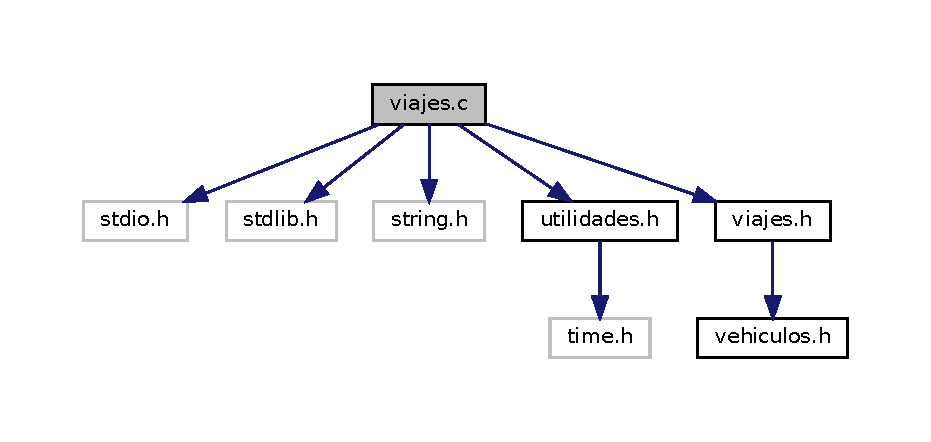
\includegraphics[width=\textwidth, angle=0]{viajes_include.pdf}
\subsection{Estructura de Datos}
\begin{itemize}
    \item \funrf{struct Viajes}{struct:viajes}
    \item \funrf{struct Pasos}{struct:pasos}
    \item \funrf{struct vViajes}{struct:viajespasos}
\end{itemize}
\subsection{Funciones}
\begin{itemize}
    \item \funrf{Viajes* initViajes(int* n)}{def:initviajes}
    \item \funrf{Pasos* initPasos(int* n)}{def:initpasos}
    \item \funrf{void publicarViajeUsuario(vViajes* v,vVehiculos* ve,int userId)}{def:puviuser}
    \item \cc{void editarViajesUsuario(vViajes* v,vVehiculos* ve,int userId)}
    \item \cc{void incorporarseViaje(vViajes *v)}
    \item \cc{void detalleViaje(vViajes* v)}
    \item \cc{void publicarViajeAdmin(vViajes *v, vVehiculos *ve)}
    \item \cc{void eliminarViajesAdmin(vViajes* v)}
    \item \cc{void modificarViajesAdmin(vViajes* v,vVehiculos *vve)}
    \item \cc{void listarViajesAdmin(vViajes* v)}
    \item \cc{void saveViajes(int n,Viajes* viajes)}
    \item \cc{void savePasos(int n,Pasos* pasos)}
    \item \cc{int buscarIndexViajes(vViajes* v,int id_viaje)}
    \item \cc{void listarViajesAbiertos(vViajes *v)}
    \item \cc{void actualizarViajes(vViajes* v)}
\end{itemize}
\subsection{Definiciones}
\begin{itemize}
    \item \label{def:initviajes}\cc{Viajes* initViajes(int* n)}
    \begin{itemize}
        \item \textbf{Descripcion}
        \begin{itemize}
			\item Inicializa una estructura del tipo Viajes.
		\end{itemize}
		\item \textbf{Parametros}
		\begin{itemize}
			\item \cc{n} $\rightarrow$ Referencia al tamaño de la estructura.
		\end{itemize}
		\item \textbf{Devuelve}
		\begin{itemize}
			\item Un vector con los datos del fichero Viajes.txt
		\end{itemize}
	\end{itemize}
    \item \label{def:initpasos}\cc{Pasos* initPasos(int* n)}
    \begin{itemize}
        \item \textbf{Descripcion}
        \begin{itemize}
			\item Inicializa una estructura del tipo Pasos.
		\end{itemize}
		\item \textbf{Parametros}
		\begin{itemize}
			\item \cc{n} $\rightarrow$ Referencia al tamaño de la estructura.
		\end{itemize}
		\item \textbf{Devuelve}
		\begin{itemize}
			\item Un vector con los datos del fichero Pasos.txt
		\end{itemize}
	\end{itemize}
    \item \label{def:puviuser}\cc{void publicarViajeUsuario(vViajes* v,vVehiculos* ve,int userId)}
    \begin{itemize}
        \item \textbf{Descripcion}
        \begin{itemize}
			\item Funcion para publicar un viaje en el sistema de esi-share.
		\end{itemize}
		\item \textbf{Parametros}
		\begin{itemize}
			\item \cc{v}  $\rightarrow$ Referencia al vector de viajes.
            \item \cc{ve} $\rightarrow$ Referencia al vector de vehiculos.
            \item \cc{userId} $\rightarrow$ Identificador del usuario que publica el viaje.
		\end{itemize}
	\end{itemize}


\end{itemize}
